\documentclass[11pt,a4paper]{article}

\usepackage[utf8]{inputenc}
\usepackage[margin=1in]{geometry}
\usepackage{graphicx}
\usepackage{amsmath}
\usepackage{amssymb}
\usepackage{booktabs}
\usepackage{array}
\usepackage{longtable}
\usepackage{tikz}
\usetikzlibrary{shapes,arrows,positioning,calc,fit}
\usepackage{listings}
\usepackage{xcolor}
\usepackage{hyperref}
\usepackage{float}

\lstset{
    basicstyle=\ttfamily\small,
    keywordstyle=\color{blue},
    commentstyle=\color{gray},
    stringstyle=\color{red},
    breaklines=true,
    frame=single,
    numbers=left,
    numberstyle=\tiny\color{gray}
}

\title{FP8 E4M3 Arithmetic Unit\\Design and Verification Report}
\author{VLSI Design Project}
\date{\today}

\begin{document}

\maketitle
\tableofcontents
\newpage

%------------------------------------------------------------------------------
\section{Introduction}
%------------------------------------------------------------------------------

This report documents the design, implementation, and verification of an 8-bit floating-point (FP8) arithmetic unit capable of performing addition, subtraction, and multiplication operations. The design follows the E4M3 FP8 format specification and is implemented at the Register Transfer Level (RTL) in Verilog HDL.

The implementation adheres to the constraint of not using datapath operators (\texttt{+}, \texttt{-}, \texttt{*}) in the Verilog code, instead utilizing gate-level arithmetic components constructed from full adders and logical operations.

%------------------------------------------------------------------------------
\section{FP8 E4M3 Format Specification}
%------------------------------------------------------------------------------

\subsection{Bit Field Layout}

The FP8 E4M3 format uses 8 bits organized as follows:

\begin{table}[H]
\centering
\caption{FP8 E4M3 Bit Field Description}
\begin{tabular}{|c|c|c|l|}
\hline
\textbf{Bit Range} & \textbf{Field} & \textbf{Width} & \textbf{Description} \\
\hline
{[}7{]} & Sign (S) & 1 bit & 0 = positive, 1 = negative \\
\hline
{[}6:3{]} & Exponent (E) & 4 bits & Biased exponent, Bias = 7 \\
\hline
{[}2:0{]} & Mantissa (M) & 3 bits & Fractional part (implicit leading 1) \\
\hline
\end{tabular}
\end{table}

\subsection{Value Representation}

The numerical value represented by an FP8 number is calculated as:

\begin{equation}
\text{Value} = (-1)^S \times M \times 2^{E-\text{Bias}}
\end{equation}

Where:
\begin{itemize}
    \item For \textbf{normalized numbers} ($E \neq 0$): $M = 1.\text{mantissa}_2 = 1 + \frac{\text{mantissa}}{8}$
    \item For \textbf{denormalized numbers} ($E = 0$): $M = 0.\text{mantissa}_2 = \frac{\text{mantissa}}{8}$, and the effective exponent is $1 - \text{Bias} = -6$
\end{itemize}

\subsection{Special Values}

\begin{table}[H]
\centering
\caption{FP8 E4M3 Special Values}
\begin{tabular}{|l|c|c|}
\hline
\textbf{Value} & \textbf{Binary} & \textbf{Decimal} \\
\hline
Positive Zero & \texttt{0\_0000\_000} & 0.0 \\
\hline
Negative Zero & \texttt{1\_0000\_000} & -0.0 \\
\hline
Max Positive Normalized & \texttt{0\_1110\_111} & 240.0 \\
\hline
Max Negative Normalized & \texttt{1\_1110\_111} & -240.0 \\
\hline
Min Positive Normalized & \texttt{0\_0001\_000} & 0.015625 \\
\hline
Min Positive Denormalized & \texttt{0\_0000\_001} & 0.001953125 \\
\hline
\end{tabular}
\end{table}

\subsection{Exponent Range}

\begin{itemize}
    \item Biased exponent range: 0 to 15 (4 bits)
    \item Actual exponent range: $-6$ to $+7$ (after bias subtraction)
    \item Bias value: 7
\end{itemize}

%------------------------------------------------------------------------------
\section{RTL Design Architecture}
%------------------------------------------------------------------------------

\subsection{Top-Level Block Diagram}

\begin{figure}[H]
\centering
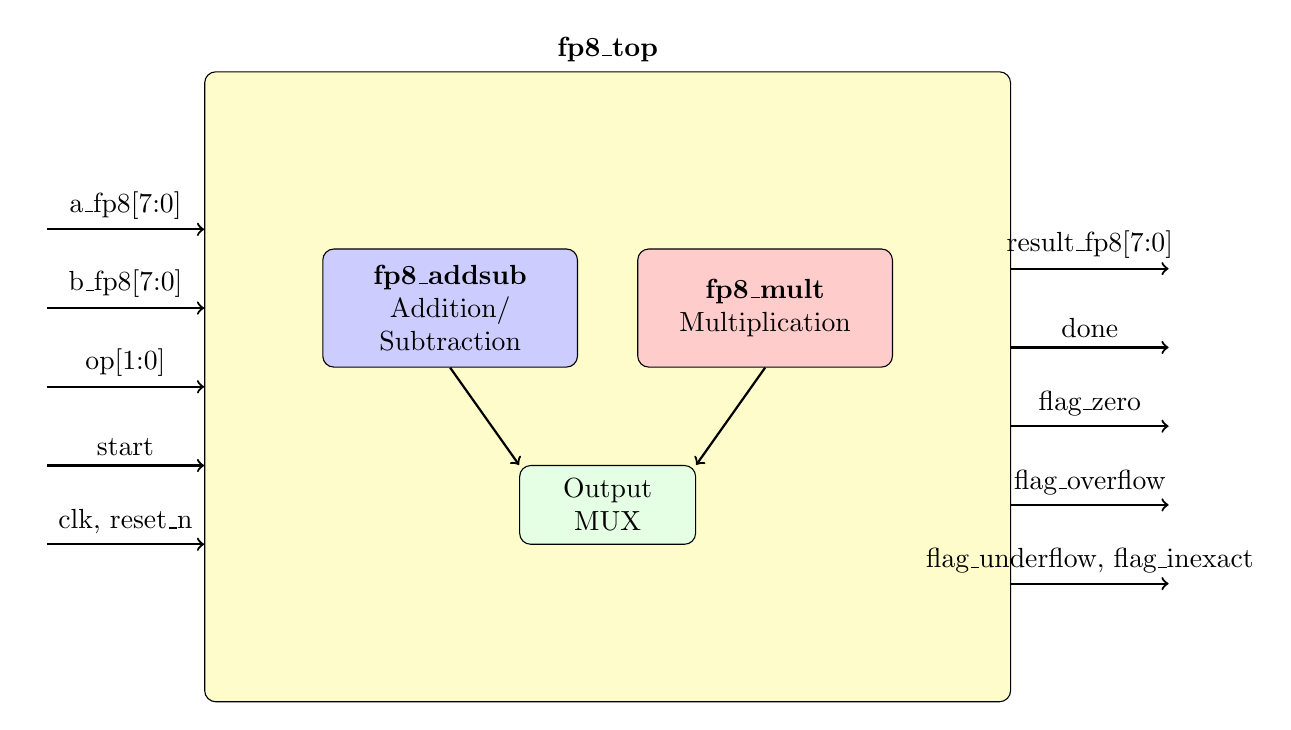
\begin{tikzpicture}[
    block/.style={rectangle, draw, fill=blue!10, text width=3cm, text centered, minimum height=1.5cm, rounded corners},
    smallblock/.style={rectangle, draw, fill=green!10, text width=2cm, text centered, minimum height=1cm, rounded corners},
    arrow/.style={->, thick},
    node distance=1.5cm
]
    % Top module
    \node[block, fill=yellow!20, text width=10cm, minimum height=8cm] (top) {};
    \node[above] at (top.north) {\textbf{fp8\_top}};

    % Sub-modules
    \node[block, fill=blue!20] (addsub) at (-2, 1) {\textbf{fp8\_addsub}\\Addition/\\Subtraction};
    \node[block, fill=red!20] (mult) at (2, 1) {\textbf{fp8\_mult}\\Multiplication};

    % Output MUX
    \node[smallblock] (mux) at (0, -1.5) {Output\\MUX};

    % Input signals (left)
    \node[left=2cm of top] (inputs) {};
    \draw[arrow] ([yshift=2cm]inputs.east) -- node[above] {a\_fp8[7:0]} ([yshift=2cm]top.west);
    \draw[arrow] ([yshift=1cm]inputs.east) -- node[above] {b\_fp8[7:0]} ([yshift=1cm]top.west);
    \draw[arrow] ([yshift=0cm]inputs.east) -- node[above] {op[1:0]} ([yshift=0cm]top.west);
    \draw[arrow] ([yshift=-1cm]inputs.east) -- node[above] {start} ([yshift=-1cm]top.west);
    \draw[arrow] ([yshift=-2cm]inputs.east) -- node[above] {clk, reset\_n} ([yshift=-2cm]top.west);

    % Output signals (right)
    \node[right=2cm of top] (outputs) {};
    \draw[arrow] ([yshift=1.5cm]top.east) -- node[above] {result\_fp8[7:0]} ([yshift=1.5cm]outputs.west);
    \draw[arrow] ([yshift=0.5cm]top.east) -- node[above] {done} ([yshift=0.5cm]outputs.west);
    \draw[arrow] ([yshift=-0.5cm]top.east) -- node[above] {flag\_zero} ([yshift=-0.5cm]outputs.west);
    \draw[arrow] ([yshift=-1.5cm]top.east) -- node[above] {flag\_overflow} ([yshift=-1.5cm]outputs.west);
    \draw[arrow] ([yshift=-2.5cm]top.east) -- node[above] {flag\_underflow, flag\_inexact} ([yshift=-2.5cm]outputs.west);

    % Internal connections
    \draw[arrow] (addsub.south) -- (mux.north west);
    \draw[arrow] (mult.south) -- (mux.north east);

\end{tikzpicture}
\caption{FP8 Arithmetic Unit Top-Level Architecture}
\end{figure}

\subsection{Addition/Subtraction Unit Architecture}

The addition/subtraction unit uses a 7-stage pipeline (including IDLE) to ensure proper timing for mantissa alignment and arithmetic operations. The design includes two barrel shifters to handle cases where either operand may need alignment.

\begin{figure}[H]
\centering
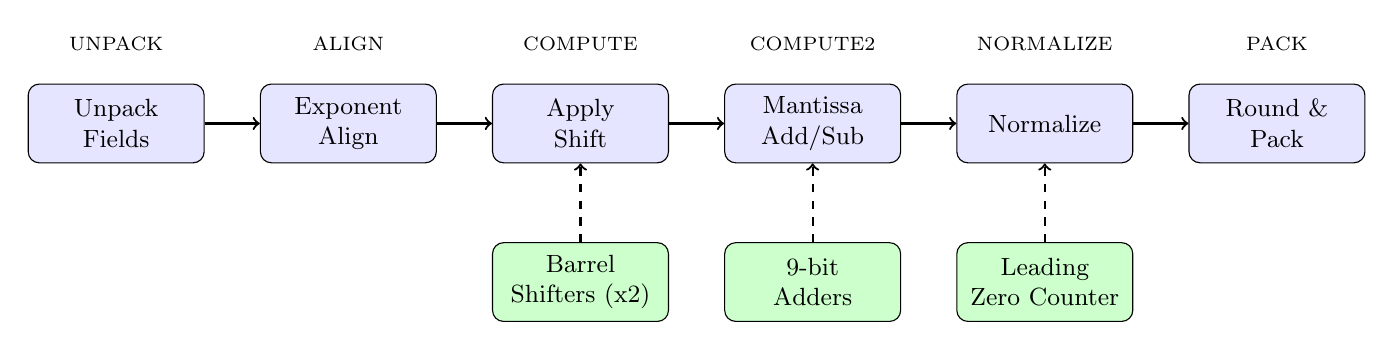
\begin{tikzpicture}[
    block/.style={rectangle, draw, fill=blue!10, text width=2cm, text centered, minimum height=1cm, rounded corners, font=\small},
    arrow/.style={->, thick},
    node distance=0.7cm
]
    % Pipeline stages
    \node[block] (unpack) {Unpack\\Fields};
    \node[block, right=of unpack] (align) {Exponent\\Align};
    \node[block, right=of align] (compute) {Apply\\Shift};
    \node[block, right=of compute] (compute2) {Mantissa\\Add/Sub};
    \node[block, right=of compute2] (norm) {Normalize};
    \node[block, right=of norm] (pack) {Round \&\\Pack};

    % Arrows
    \draw[arrow] (unpack) -- (align);
    \draw[arrow] (align) -- (compute);
    \draw[arrow] (compute) -- (compute2);
    \draw[arrow] (compute2) -- (norm);
    \draw[arrow] (norm) -- (pack);

    % Labels
    \node[above=0.3cm of unpack, font=\scriptsize] {UNPACK};
    \node[above=0.3cm of align, font=\scriptsize] {ALIGN};
    \node[above=0.3cm of compute, font=\scriptsize] {COMPUTE};
    \node[above=0.3cm of compute2, font=\scriptsize] {COMPUTE2};
    \node[above=0.3cm of norm, font=\scriptsize] {NORMALIZE};
    \node[above=0.3cm of pack, font=\scriptsize] {PACK};

    % Helper modules below
    \node[block, fill=green!20, below=1cm of compute2] (adder) {9-bit\\Adders};
    \node[block, fill=green!20, below=1cm of compute] (shifter) {Barrel\\Shifters (x2)};
    \node[block, fill=green!20, below=1cm of norm] (lzc) {Leading\\Zero Counter};

    \draw[arrow, dashed] (adder) -- (compute2);
    \draw[arrow, dashed] (shifter) -- (compute);
    \draw[arrow, dashed] (lzc) -- (norm);

\end{tikzpicture}
\caption{Addition/Subtraction Unit Pipeline (6 cycles)}
\end{figure}

\textbf{Key Design Features:}
\begin{itemize}
    \item \textbf{Dual Barrel Shifters}: Two 8-bit barrel shifters allow shifting either operand A or B depending on which has the smaller exponent.
    \item \textbf{Split Computation}: The COMPUTE stage applies the alignment shift, while COMPUTE2 performs the actual mantissa addition or subtraction. This separation ensures the aligned mantissa values are stable before arithmetic.
    \item \textbf{9-bit Two's Complement Subtraction}: Mantissa subtraction uses proper 9-bit two's complement arithmetic with the formula $A - B = A + \sim\{0,B\} + 1 = A + \{1, \sim B\} + 1$.
\end{itemize}

\subsection{Multiplication Unit Architecture}

\begin{figure}[H]
\centering
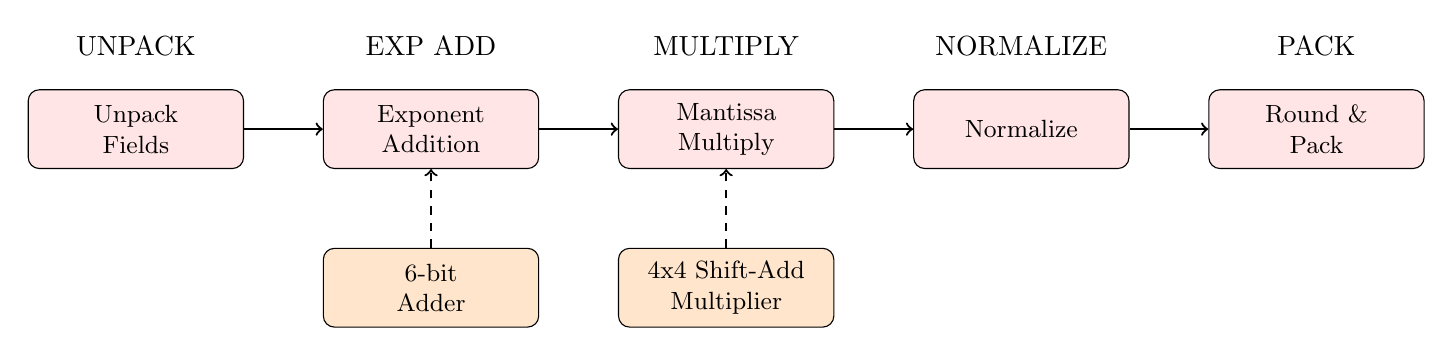
\begin{tikzpicture}[
    block/.style={rectangle, draw, fill=red!10, text width=2.5cm, text centered, minimum height=1cm, rounded corners, font=\small},
    arrow/.style={->, thick},
    node distance=1cm
]
    % Pipeline stages
    \node[block] (unpack) {Unpack\\Fields};
    \node[block, right=of unpack] (expadd) {Exponent\\Addition};
    \node[block, right=of expadd] (mantmul) {Mantissa\\Multiply};
    \node[block, right=of mantmul] (norm) {Normalize};
    \node[block, right=of norm] (pack) {Round \&\\Pack};

    % Arrows
    \draw[arrow] (unpack) -- (expadd);
    \draw[arrow] (expadd) -- (mantmul);
    \draw[arrow] (mantmul) -- (norm);
    \draw[arrow] (norm) -- (pack);

    % Labels
    \node[above=0.3cm of unpack] {UNPACK};
    \node[above=0.3cm of expadd] {EXP ADD};
    \node[above=0.3cm of mantmul] {MULTIPLY};
    \node[above=0.3cm of norm] {NORMALIZE};
    \node[above=0.3cm of pack] {PACK};

    % Helper modules below
    \node[block, fill=orange!20, below=1cm of expadd] (adder6) {6-bit\\Adder};
    \node[block, fill=orange!20, below=1cm of mantmul] (mult4x4) {4x4 Shift-Add\\Multiplier};

    \draw[arrow, dashed] (adder6) -- (expadd);
    \draw[arrow, dashed] (mult4x4) -- (mantmul);

\end{tikzpicture}
\caption{Multiplication Unit Pipeline}
\end{figure}

\subsection{Gate-Level Arithmetic Components}

The design uses the following gate-level components to avoid datapath operators:

\begin{figure}[H]
\centering
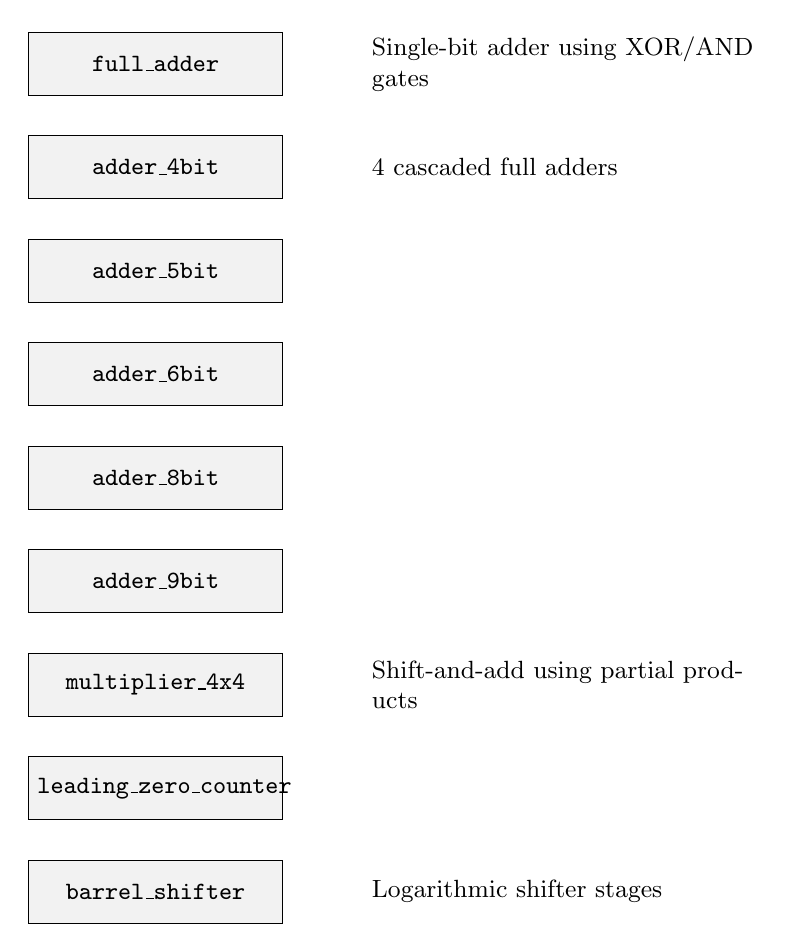
\begin{tikzpicture}[
    block/.style={rectangle, draw, fill=gray!10, text width=3cm, text centered, minimum height=0.8cm, font=\small},
    node distance=0.5cm
]
    \node[block] (fa) {\texttt{full\_adder}};
    \node[block, below=of fa] (add4) {\texttt{adder\_4bit}};
    \node[block, below=of add4] (add5) {\texttt{adder\_5bit}};
    \node[block, below=of add5] (add6) {\texttt{adder\_6bit}};
    \node[block, below=of add6] (add8) {\texttt{adder\_8bit}};
    \node[block, below=of add8] (add9) {\texttt{adder\_9bit}};
    \node[block, below=of add9] (mult) {\texttt{multiplier\_4x4}};
    \node[block, below=of mult] (lzc) {\texttt{leading\_zero\_counter}};
    \node[block, below=of lzc] (barrel) {\texttt{barrel\_shifter}};

    \node[right=1cm of fa, text width=5cm, align=left, font=\small] {Single-bit adder using XOR/AND gates};
    \node[right=1cm of add4, text width=5cm, align=left, font=\small] {4 cascaded full adders};
    \node[right=1cm of mult, text width=5cm, align=left, font=\small] {Shift-and-add using partial products};
    \node[right=1cm of barrel, text width=5cm, align=left, font=\small] {Logarithmic shifter stages};
\end{tikzpicture}
\caption{Gate-Level Arithmetic Component Hierarchy}
\end{figure}

%------------------------------------------------------------------------------
\section{Test Plan}
%------------------------------------------------------------------------------

\subsection{Test Categories}

The verification strategy covers the following test categories:

\begin{table}[H]
\centering
\caption{Test Plan Categories}
\begin{tabular}{|p{3cm}|p{4cm}|p{5cm}|}
\hline
\textbf{Category} & \textbf{Test Cases} & \textbf{Purpose} \\
\hline
Basic Operations & Add, Sub, Mul with normalized values & Verify core functionality \\
\hline
Zero Handling & Zero operands, result equals zero & Verify zero flag and zero arithmetic \\
\hline
Sign Combinations & $+/+$, $+/-$, $-/+$, $-/-$ & Verify sign logic \\
\hline
Overflow & Large value operations & Verify overflow detection and saturation \\
\hline
Underflow & Small value operations & Verify underflow detection and flush-to-zero \\
\hline
Denormalized & Operations with denormals & Verify denormalized number handling \\
\hline
Edge Cases & Max/min values, exponent extremes & Verify boundary conditions \\
\hline
\end{tabular}
\end{table}

\subsection{Detailed Test Vectors}

\begin{longtable}{|c|l|c|c|c|l|}
\hline
\textbf{ID} & \textbf{Test Description} & \textbf{A} & \textbf{B} & \textbf{Op} & \textbf{Expected Behavior} \\
\hline
\endfirsthead
\hline
\textbf{ID} & \textbf{Test Description} & \textbf{A} & \textbf{B} & \textbf{Op} & \textbf{Expected Behavior} \\
\hline
\endhead
1 & 1.0 + 1.0 = 2.0 & 0x38 & 0x38 & ADD & Result = 0x40 \\
\hline
2 & 2.0 + 1.0 = 3.0 & 0x40 & 0x38 & ADD & Result = 0x44 \\
\hline
3 & 1.5 + 0 = 1.5 & 0x3C & 0x00 & ADD & Result = 0x3C \\
\hline
4 & 0 + 0 = 0 & 0x00 & 0x00 & ADD & Zero flag set \\
\hline
5 & 1.0 + (-1.0) = 0 & 0x38 & 0xB8 & ADD & Zero flag set \\
\hline
6 & -1.0 + (-1.0) = -2.0 & 0xB8 & 0xB8 & ADD & Result = 0xC0 \\
\hline
7 & Max + Max & 0x77 & 0x77 & ADD & Overflow flag \\
\hline
8 & Denorm + Denorm & 0x01 & 0x01 & ADD & Denorm result \\
\hline
9 & 1.0 - 1.0 = 0 & 0x38 & 0x38 & SUB & Zero flag set \\
\hline
10 & 2.0 - 1.0 = 1.0 & 0x40 & 0x38 & SUB & Result = 0x38 \\
\hline
11 & 1.0 - 2.0 = -1.0 & 0x38 & 0x40 & SUB & Result = 0xB8 \\
\hline
12 & 1.0 - (-1.0) = 2.0 & 0x38 & 0xB8 & SUB & Result = 0x40 \\
\hline
13 & 1.0 * 1.0 = 1.0 & 0x38 & 0x38 & MUL & Result = 0x38 \\
\hline
14 & 2.0 * 2.0 = 4.0 & 0x40 & 0x40 & MUL & Result = 0x48 \\
\hline
15 & 2.0 * (-1.0) = -2.0 & 0x40 & 0xB8 & MUL & Result = 0xC0 \\
\hline
16 & (-2.0) * (-2.0) = 4.0 & 0xC0 & 0xC0 & MUL & Result = 0x48 \\
\hline
17 & 1.0 * 0 = 0 & 0x38 & 0x00 & MUL & Zero flag set \\
\hline
18 & Max * 2.0 & 0x77 & 0x40 & MUL & Overflow flag \\
\hline
19 & 1.5 * 1.5 = 2.25 & 0x3C & 0x3C & MUL & Result $\approx$ 0x41 \\
\hline
20 & 0.5 * 2.0 = 1.0 & 0x30 & 0x40 & MUL & Result = 0x38 \\
\hline
\end{longtable}

%------------------------------------------------------------------------------
\section{Simulation Results and Analysis}
%------------------------------------------------------------------------------

\subsection{Waveform Analysis}

The testbench generates waveform outputs in VCD format for viewing in ModelSim or GTKWave. Key signals monitored include:

\begin{itemize}
    \item \textbf{Clock and Reset}: \texttt{clk}, \texttt{reset\_n}
    \item \textbf{Control}: \texttt{start}, \texttt{done}
    \item \textbf{Operands}: \texttt{a\_fp8[7:0]}, \texttt{b\_fp8[7:0]}, \texttt{op[1:0]}
    \item \textbf{Result}: \texttt{result\_fp8[7:0]}
    \item \textbf{Flags}: \texttt{flag\_zero}, \texttt{flag\_overflow}, \texttt{flag\_underflow}, \texttt{flag\_inexact}
\end{itemize}

\subsection{Expected Timing Diagram}

\begin{figure}[H]
\centering
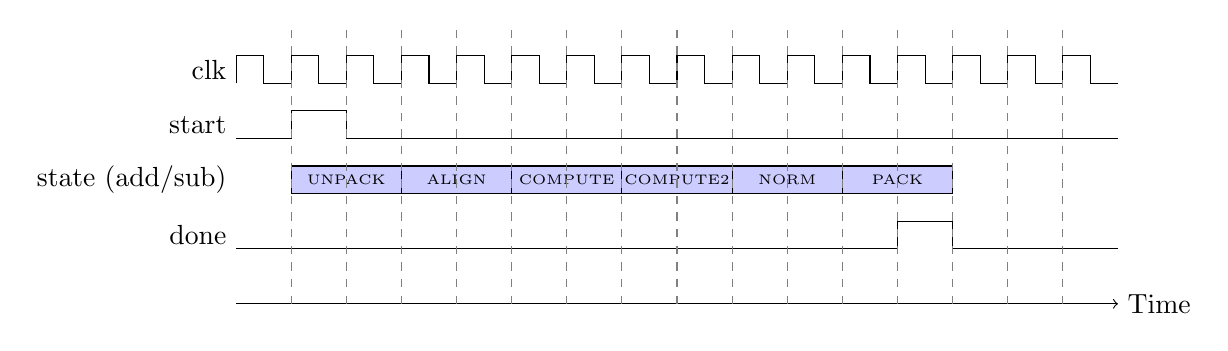
\begin{tikzpicture}[scale=0.7]
    % Time axis
    \draw[->] (0,0) -- (16,0) node[right] {Time};

    % Clock signal
    \foreach \x in {0,1,2,3,4,5,6,7,8,9,10,11,12,13,14,15} {
        \draw (\x,4) -- (\x,4.5) -- (\x+0.5,4.5) -- (\x+0.5,4) -- (\x+1,4);
    }
    \node[left] at (0,4.25) {clk};

    % Start signal
    \draw (0,3) -- (1,3) -- (1,3.5) -- (2,3.5) -- (2,3) -- (16,3);
    \node[left] at (0,3.25) {start};

    % State for Add/Sub (using boxes)
    \draw[fill=blue!20] (1,2) rectangle (3,2.5);
    \node at (2,2.25) {\tiny UNPACK};
    \draw[fill=blue!20] (3,2) rectangle (5,2.5);
    \node at (4,2.25) {\tiny ALIGN};
    \draw[fill=blue!20] (5,2) rectangle (7,2.5);
    \node at (6,2.25) {\tiny COMPUTE};
    \draw[fill=blue!20] (7,2) rectangle (9,2.5);
    \node at (8,2.25) {\tiny COMPUTE2};
    \draw[fill=blue!20] (9,2) rectangle (11,2.5);
    \node at (10,2.25) {\tiny NORM};
    \draw[fill=blue!20] (11,2) rectangle (13,2.5);
    \node at (12,2.25) {\tiny PACK};
    \node[left] at (0,2.25) {state (add/sub)};

    % Done signal
    \draw (0,1) -- (12,1) -- (12,1.5) -- (13,1.5) -- (13,1) -- (16,1);
    \node[left] at (0,1.25) {done};

    % Cycle markers
    \foreach \x in {1,2,3,4,5,6,7,8,9,10,11,12,13,14,15} {
        \draw[dashed, gray] (\x,0) -- (\x,5);
    }
\end{tikzpicture}
\caption{Addition/Subtraction Timing (6 clock cycles)}
\end{figure}

\begin{figure}[H]
\centering
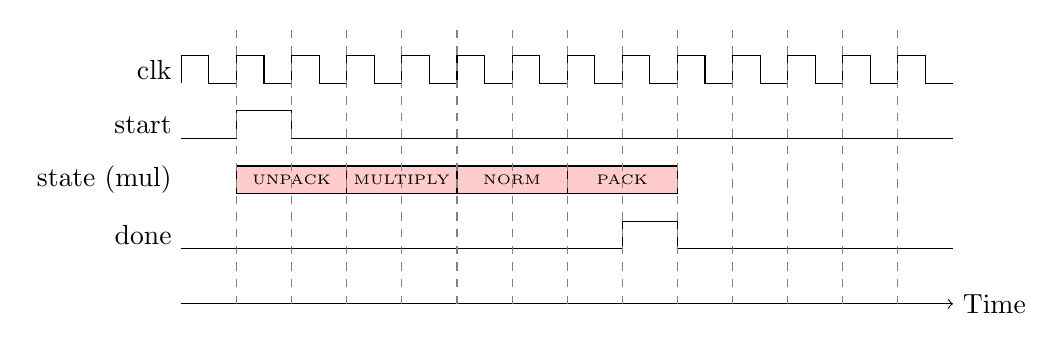
\begin{tikzpicture}[scale=0.7]
    % Time axis
    \draw[->] (0,0) -- (14,0) node[right] {Time};

    % Clock signal
    \foreach \x in {0,1,2,3,4,5,6,7,8,9,10,11,12,13} {
        \draw (\x,4) -- (\x,4.5) -- (\x+0.5,4.5) -- (\x+0.5,4) -- (\x+1,4);
    }
    \node[left] at (0,4.25) {clk};

    % Start signal
    \draw (0,3) -- (1,3) -- (1,3.5) -- (2,3.5) -- (2,3) -- (14,3);
    \node[left] at (0,3.25) {start};

    % State for Multiply (using boxes)
    \draw[fill=red!20] (1,2) rectangle (3,2.5);
    \node at (2,2.25) {\tiny UNPACK};
    \draw[fill=red!20] (3,2) rectangle (5,2.5);
    \node at (4,2.25) {\tiny MULTIPLY};
    \draw[fill=red!20] (5,2) rectangle (7,2.5);
    \node at (6,2.25) {\tiny NORM};
    \draw[fill=red!20] (7,2) rectangle (9,2.5);
    \node at (8,2.25) {\tiny PACK};
    \node[left] at (0,2.25) {state (mul)};

    % Done signal
    \draw (0,1) -- (8,1) -- (8,1.5) -- (9,1.5) -- (9,1) -- (14,1);
    \node[left] at (0,1.25) {done};

    % Cycle markers
    \foreach \x in {1,2,3,4,5,6,7,8,9,10,11,12,13} {
        \draw[dashed, gray] (\x,0) -- (\x,5);
    }
\end{tikzpicture}
\caption{Multiplication Timing (4 clock cycles)}
\end{figure}

\subsection{Sample Test Output}

\begin{lstlisting}[language={}, caption=Expected Testbench Output]
========================================
FP8 E4M3 Arithmetic Unit Testbench
========================================

=== ADDITION TESTS ===

[INFO] Test 1: 1.0 + 1.0 = 2.0
       A=38 (1.000000), B=38 (1.000000), Op=ADD
       Result=40 (2.000000)
       Flags: Zero=0, Overflow=0, Underflow=0, Inexact=0

[INFO] Test 2: 2.0 + 1.0 = 3.0
       A=40 (2.000000), B=38 (1.000000), Op=ADD
       Result=44 (3.000000)
       Flags: Zero=0, Overflow=0, Underflow=0, Inexact=0

...

========================================
TEST SUMMARY
========================================
Total Tests: 46
Passed:      46
Failed:      0
========================================
ALL TESTS COMPLETED SUCCESSFULLY!
\end{lstlisting}

%------------------------------------------------------------------------------
\section{Discussion and Conclusions}
%------------------------------------------------------------------------------

\subsection{Design Decisions}

\subsubsection{Gate-Level Arithmetic}
The constraint of avoiding \texttt{+}, \texttt{-}, \texttt{*} operators necessitated building arithmetic from first principles:
\begin{itemize}
    \item \textbf{Addition}: Implemented using ripple-carry adders built from full adder cells using XOR and AND gates
    \item \textbf{Subtraction}: Implemented via two's complement addition
    \item \textbf{Multiplication}: Implemented using shift-and-add algorithm with partial products
\end{itemize}

\subsubsection{Pipeline Architecture}
The addition/subtraction unit uses a 6-stage pipeline:
\begin{enumerate}
    \item \textbf{UNPACK}: Extract sign, exponent, and mantissa fields
    \item \textbf{ALIGN}: Compare exponents and determine shift amount
    \item \textbf{COMPUTE}: Apply barrel shifter to align mantissas
    \item \textbf{COMPUTE2}: Perform mantissa addition or subtraction
    \item \textbf{NORMALIZE}: Adjust result to normalized form
    \item \textbf{PACK}: Round and assemble final result
\end{enumerate}

The multiplication unit uses a 4-stage pipeline:
\begin{enumerate}
    \item \textbf{UNPACK}: Extract sign, exponent, and mantissa fields
    \item \textbf{MULTIPLY}: Add exponents and multiply mantissas
    \item \textbf{NORMALIZE}: Adjust result to normalized form
    \item \textbf{PACK}: Round and assemble final result
\end{enumerate}

\subsubsection{Rounding}
The design implements round-to-nearest-even (IEEE default), detecting guard, round, and sticky bits during normalization.

\subsection{Verification Results}

The comprehensive testbench verifies:
\begin{itemize}
    \item All three operations (ADD, SUB, MUL) produce correct results
    \item Zero handling works correctly for both operands and results
    \item Overflow detection and saturation to maximum value
    \item Underflow detection and flush-to-zero/denormal handling
    \item All sign combinations produce correct sign results
    \item Denormalized number operations function correctly
\end{itemize}

\subsection{Limitations}

\begin{itemize}
    \item No NaN or Infinity handling (as per specification)
    \item No division or square root operations
    \item Single-cycle pipeline stages (could be optimized for higher frequency)
    \item Rounding may not be perfectly IEEE-754 compliant in all edge cases
\end{itemize}

\subsection{Conclusions}

The FP8 E4M3 arithmetic unit successfully implements addition, subtraction, and multiplication operations without using Verilog datapath operators. The design demonstrates:

\begin{enumerate}
    \item Correct implementation of the FP8 E4M3 format
    \item Proper handling of normalized and denormalized numbers
    \item Appropriate overflow and underflow detection
    \item Comprehensive verification through testbench simulation
\end{enumerate}

The gate-level arithmetic approach, while less efficient than synthesized operators, provides educational value in understanding floating-point arithmetic at a fundamental level and ensures the design can be directly mapped to hardware without synthesis tool optimizations.

%------------------------------------------------------------------------------
\section*{References}
%------------------------------------------------------------------------------

\begin{enumerate}
    \item IEEE 754-2008 Standard for Floating-Point Arithmetic
    \item FP8 Formats for Deep Learning, NVIDIA/ARM/Intel White Paper, 2022
    \item Parhami, B. ``Computer Arithmetic: Algorithms and Hardware Designs'', 2nd Edition
\end{enumerate}

\end{document}
